\documentclass{beamer}

%\usepackage{multimedia}

% For more themes, color themes and font themes, see:
% http://deic.uab.es/~iblanes/beamer_gallery/index_by_theme.html
%
\mode<presentation>
{
  \usetheme{Madrid}       % or try default, Darmstadt, Warsaw, ...
  \usecolortheme{seagull} % or try albatross, beaver, crane, ...
  \usefonttheme{serif}    % or try default, structurebold, ...
  \setbeamertemplate{navigation symbols}{}
  \setbeamertemplate{caption}[numbered]
	\setbeamertemplate{footline}{}
	\setbeamersize{text margin right=2pt}
} 

\usepackage{tikz}
\usetikzlibrary{decorations.markings,angles}
\usepackage{tikz-3dplot} 

\usepackage{amsmath}


\begin{document}

\begin{frame}{Light bridge profiles. Two magnetic components}
\begin{itemize}
\item double-peaked shape of the blue component $\implies$ two distinct magnetic components 
in the resolution element (not completely spatially resolved)
\begin{itemize}
\item {\bf strong} magnetic field (3200 G) - corresponding to the surrounding umbra - inclined by 40$^{\circ}$ to LOS
\item{\bf weak} magnetic field component (1800 G) inclined by 60$^{\circ}$ to LOS
\end{itemize}
\item asymmetry of the profile $\implies$ velocity shift between them:
the weak field component red-shifted by 1.1 km/s relative to the strong-field component
\end{itemize}

\end{frame}

\begin{frame}{Light bridge profiles. Fe 15648.5 $\AA$ Stokes I}

\begin{figure}[H]
 \centering
 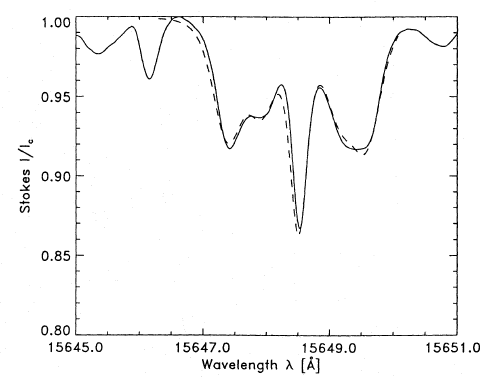
\includegraphics[scale=0.4]{stokesI.png}
\caption{Stokes I profile of FeI 15648.5 $\AA$ observed in the light bridge (solid curve) and the fit using
a model composed by two magnetic components (dashed line)}
\end{figure}
\end{frame}

\begin{frame}{Light bridge profiles. Fitting the two components}
\begin{itemize}
\item the final synthetic profile (dashed line from the Figure) is compounded by 45\% weak + 55\% strong 
{\bf if they have the same continuum intensity}
\item taking into account the different continuum intensity:  30\% weak + 70\% strong
\item all four light-bridge profiles required a combination of this kind in order to fit the data:
\begin{itemize}
\item strong field component between 2900 and 3200 G, inclined by 40$^{\circ}$ to LOS, contribution 65-70\%
\item the weak field component between 1800 and 1900 G, inclined by an angle between 60$^{\circ}$ and 70$^{\circ}$
to LOS, contribution 30-35\% 
\end{itemize}
\item two out of four cases present a shift between the two components: the weak field red-shifted against the strong field, 
and the maximum shift observed: 1.5 km/s
\end{itemize}
\end{frame}

\begin{frame}{Blend at 15648.5 $\AA$. }
\begin{itemize}
\item {\bf Blue component}: a shoulder (blend from another iron line at 15647.4 $\AA$) which matches exactly on the blue component for 
a magnetic field B = 3200 G.
This means that for fields B $\lessapprox$ 3200 G, the asymmetry increases with the magnetic field.
\item {\bf Red component}: weaker blend (located closer to the $\pi$ component) responsible for the width of the component.
\end{itemize}
\begin{itemize}
\item The blends are only slightly Zeeman sensitive $\implies$ a much smaller effect on {\bf Stokes V} profile.
\item For smaller filling factor or more stray light the effects of the blends on {\bf Stokes I} are larger, because the 
$\sigma$ components are weaker in this case. Only asymmetries (in Stokes I profile) for a high filling factor should be interpreted
in terms of velocity gradients.
\end{itemize}
\end{frame}

\begin{frame}{Blend at 15648.5 $\AA$. B = 1600 G}
\begin{figure}[H]
 \centering
 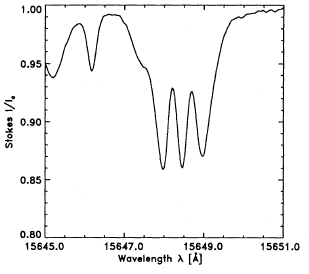
\includegraphics[scale=0.8]{stokesI-2.png}
\end{figure}
\end{frame}
\begin{frame}{Blend at 15648.5 $\AA$. B = 2380 G}
\begin{figure}[H]
 \centering
 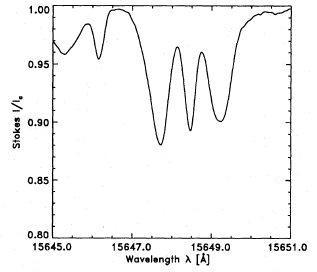
\includegraphics[scale=0.8]{stokesI-3.png}
\end{figure}
\end{frame}
\begin{frame}{Blend at 15648.5 $\AA$. B = 3040 G}
\begin{figure}[H]
 \centering
 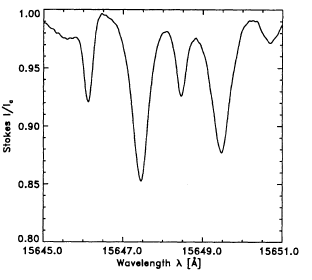
\includegraphics[scale=0.8]{stokesI-4.png}
\end{figure}
\end{frame}
\end{document}
